\documentclass[tikz,border=2pt]{standalone}
% Preámbulo común de los diagramas TikZ (misma paleta y letra que las notas)
\usepackage[T1]{fontenc}\usepackage[utf8]{inputenc}
\usepackage{libertinus}\usepackage{libertinust1math}
\usepackage[defaultsans,scale=0.92]{lato}
\usepackage{amsmath,amssymb,bm}
\usepackage{tikz}\usetikzlibrary{calc,positioning,arrows.meta,shapes.geometric,decorations.pathreplacing,decorations.pathmorphing,fit,backgrounds}
\definecolor{snlazul}{HTML}{1E5AA8}\definecolor{snlnoche}{HTML}{14213D}\definecolor{snlvioleta}{HTML}{6C4AB6}
\definecolor{snlcoral}{HTML}{D1495B}\definecolor{snlambar}{HTML}{E09F3E}\definecolor{snlverde}{HTML}{2A9D8F}
\definecolor{snlteal}{HTML}{0F7173}\definecolor{snlgris}{HTML}{5C677D}\definecolor{snlfondo}{HTML}{F4F6FA}
\tikzset{>={Stealth[length=2.2mm]},
  bloque/.style={draw=#1,fill=#1!8,thick,rounded corners=2pt,minimum height=11mm,minimum width=20mm,align=center,font=\small},
  bloque/.default=snlazul,
  suma/.style={draw=snlnoche,thick,circle,inner sep=0pt,minimum size=5mm},
  flecha/.style={->,thick,draw=snlnoche},
  etq/.style={font=\small,text=snlnoche},
  nota/.style={font=\footnotesize\sffamily,text=snlgris,align=center}}

\begin{document}
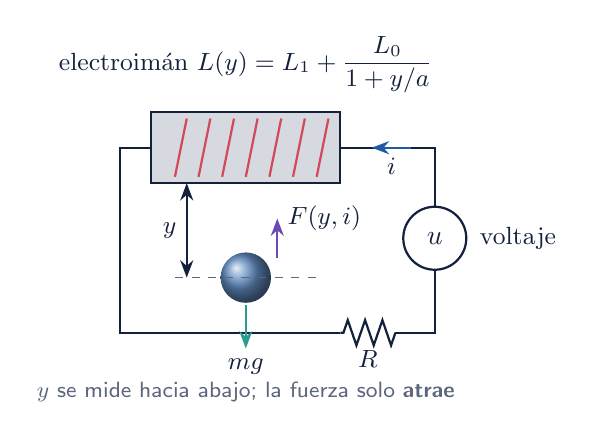
\begin{tikzpicture}
 % electroimán
 \fill[snlgris!25] (-1.2,0) rectangle (1.2,0.9);
 \draw[snlnoche,thick] (-1.2,0) rectangle (1.2,0.9);
 \foreach \x in {-0.9,-0.6,...,0.9} \draw[snlcoral,thick] (\x,0.08) -- (\x+0.15,0.82);
 \node[etq] at (0,1.5) {electroimán $L(y)=L_1+\dfrac{L_0}{1+y/a}$};
 % circuito
 \draw[thick,snlnoche] (1.2,0.45) -- (2.4,0.45) -- (2.4,-0.3);
 \draw[thick,snlnoche] (2.4,-1.1) -- (2.4,-1.9) -- (1.9,-1.9);
 \draw[thick,snlnoche,fill=white] (2.4,-0.7) circle (0.4) node {$u$};
 \node[etq,right] at (2.85,-0.7) {voltaje};
 \draw[snlnoche,thick,decorate,decoration={zigzag,amplitude=1.6mm,segment length=2.2mm}] (1.9,-1.9) -- (1.2,-1.9);
 \node[etq,below] at (1.55,-2.0) {$R$};
 \draw[thick,snlnoche] (1.2,-1.9) -- (-1.6,-1.9) -- (-1.6,0.45) -- (-1.2,0.45);
 \draw[->,thick,snlazul] (2.1,0.45) -- node[below,etq]{$i$} (1.6,0.45);
 % esfera
 \shade[ball color=snlazul!70] (0,-1.2) circle (0.32);
 \draw[dashed,snlgris] (-0.9,-1.2) -- (0.9,-1.2);
 \draw[<->,thick,snlnoche] (-0.75,0) -- node[left,etq]{$y$} (-0.75,-1.2);
 \draw[->,thick,snlverde] (0,-1.55) -- ++(0,-0.55) node[below,etq]{$mg$};
 \draw[->,thick,snlvioleta] (0.4,-0.95) -- ++(0,0.5) node[right,etq]{$F(y,i)$};
 \node[nota] at (0,-2.65) {$y$ se mide hacia abajo; la fuerza solo \textbf{atrae}};
\end{tikzpicture}
\end{document}
